% \section{Supplementary Material}

\section{Datasets}

\paragraph{Minecraft VPT}

We use the OpenAI VPT dataset of contractor gameplay \citep{vpt} and combine the available subsets 6--10, resulting in 2541 hours of gameplay.
We split the dataset into 90\% training and 10\% evaluation data, ensuring that the splits do not share any of the same underlying 5-min recording chunks.
We encode keyboard actions as a vector of binary variables and process the mouse actions as in VPT by $\mu$-law encoding, discretizing into 11 bins per coordinate, and enumerating all $11 \times 11 = 121$ combinations to obtain a categorical variable.
The image resolution is $360 \times 640$ and the framerate is 20 FPS.
We zero pad the frames to $384 \times 640$ and then patchify with patch size $16 \times 16$ into 960 tokens.
We reshape the $(N_\mathrm{b} = 512) \times (D_\mathrm{b} = 16)$ bottleneck of the tokenizer to $(N_\mathrm{z} = 256) \times 32$ for the dynamics model.
We train the dynamics model with $N_\mathrm{z} = 256$ spatial tokens, context length $C = 192$, and batch lengths $T_1 = 64$ and $T_2 = 256$.

\paragraph{Minecraft Overworld and Nether split}

To study out-of-distribution generalization of action conditioning in \method, we carefully split the Minecraft dataset into videos of the Overworld versus the Nether dimension.
We also include the End dimension into the Nether portion of the dataset.
Both the Nether and the End feature unique visuals, blocks, and terrain shapes compared to the Overworld.
The Overworld includes natural landscapes with forests, deserts, oceans, and more, whereas the Nether is underworld-themed with red blocks and lava and the End is a space-themed region.
To separate the dataset, we want to ensure no leakage from players entering the Nether/End dimensions and bringing blocks from there back to the Overworld.
For this reason, we exclude the VPT 6 and 7 subsets, which contain long free play.
We then assigned each 5 min recording of the remaining dataset to either the Overworld or the Nether/End portion based on item events that are provided by the dataset.
Whenever a Nether/End item was interacted with, we assign that video to the Nether/End split.
This ensures that the Overworld split contains no Nether/End episodes, whereas the Nether/End split can sometimes contain some Overworld episodes, although this was rare in practice.
We manually investigated the Overworld split obtained by this strategy and found no Nether/End trajectories in it.

\paragraph{SOAR Robotics}

The SOAR dataset \citep{soar} contains teleoperated demonstrations and online trajectories of a reinforcement learning policy, thus covering both successes and failures.
We split the dataset into 90\% training and 10\% evaluation data.
The dataset contains a total of 180 hours of videos with 7D relative end-effector actions.
The image resolution is $256 \times 256$ and the framerate is 5 FPS.
We patchify with patch size $16 \times 16$ into 256 tokens.
We train the dynamics model with $N_\mathrm{z} = 512$ spatial tokens, context length $C = 96$, and batch lengths $T_1 = 32$ and $T_2 = 128$.

\paragraph{Epic Kitchens}

The Epic Kitchens 100 dataset \citep{epickitchens} contains 100 hours of video from the first-person perspective of humans across 45 kitchens.
The test set contains different tasks performed in the same kitchens.
We use the dataset at $256 \times 256$ resolution and 10 FPS.
We patchify with patch size $16 \times 16$ into 256 tokens.
We train the dynamics model with $N_\mathrm{z} = 512$ spatial tokens, context length $C = 96$, and batch lengths $T_1 = 32$ and $T_2 = 128$.

\clearpage
\section{Kitchen Generations}
\vfill
\begin{figure}[t!]
\vspace*{-2\baselineskip}
\centering
\begin{subfigure}[t]{0.45\textwidth}
\centering
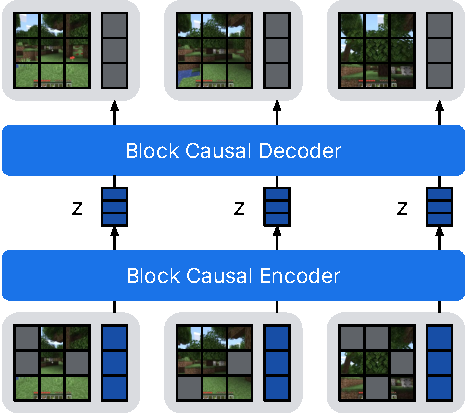
\includegraphics[height=2.4in]{figures/method/tok}
\caption{Causal Tokenizer}
\end{subfigure}%
\hfill%
\begin{subfigure}[t]{0.45\textwidth}
\centering
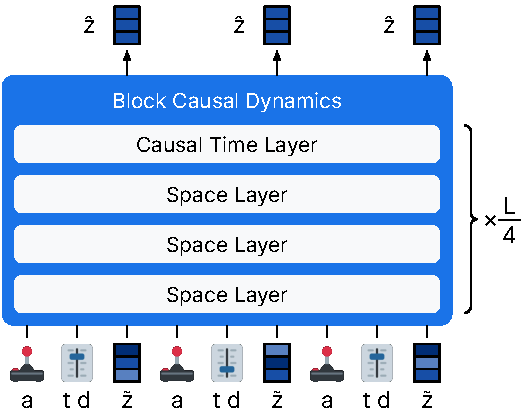
\includegraphics[height=2.5in]{figures/method/dyn}
\caption{Interactive Dynamics}
\end{subfigure}
\caption{World model design.
\method consists of a causal tokenizer and an interactive dynamics model, which both use the same block-causal transformer architecture.
The tokenizer encodes partially masked image patches and latent tokens, squeezes the latents through a low-dimensional projection with tanh activation, and decodes the patches.
It uses causal attention to achieve temporal compression while allowing frames to be decoded one by one.
The dynamics model operates on the interleaved sequence of actions, shortcut noise levels and step sizes, and tokenizer representations.
It denoises representations via a shortcut forcing objective.
After pretraining, the world model is finetuned into an agent by inserting task tokens into the dynamics transformer and predicting actions, rewards, and values from them.
}
\label{fig:model}
\end{figure}
\vfill

\section{Minecraft Tasks}
\vspace*{-2ex}
\begin{minipage}[t]{0.48\textwidth}
\centering
\vspace*{1ex}
\begin{mytabular}{
  colspec = {| C{3em} | L{13em} |},
  row{1} = {font=\bfseries},
}

\toprule
Index & Task \\
\midrule
  1 & \texttt{mine\_log} \\
  2 & \texttt{mine\_cobblestone} \\
  3 & \texttt{mine\_iron\_ore} \\
  4 & \texttt{mine\_coal} \\
  5 & \texttt{mine\_diamond} \\
  6 & \texttt{craft\_planks} \\
  7 & \texttt{craft\_stick} \\
  8 & \texttt{craft\_crafting\_table} \\
  9 & \texttt{craft\_furnace} \\
 10 & \texttt{craft\_iron\_ingot} \\
 11 & \texttt{craft\_wooden\_pickaxe} \\
 12 & \texttt{craft\_stone\_pickaxe} \\
 13 & \texttt{craft\_iron\_pickaxe} \\
 14 & \texttt{open\_crafting\_table} \\
 15 & \texttt{open\_furnace} \\
 16 & \texttt{place\_crafting\_table} \\
 17 & \texttt{place\_furnace} \\
 18 & \texttt{use\_wooden\_pickaxe} \\
 19 & \texttt{use\_stone\_pickaxe} \\
 20 & \texttt{use\_iron\_pickaxe} \\
\bottomrule

\end{mytabular}
\captionof{table}{Taskset for training the multi-task agent.}
\label{tab:mc_tasks}

\vspace*{3ex}
\centering
\newcommand{\icon}[1]{\includegraphics[height=2.5ex]{icons/#1.png}}
\newcommand{\name}[1]{\raisebox{.4ex}{#1}}
\vspace*{1ex}
\begin{mytabular}{
  colspec = {| C{3em} | L{13em} |},
  row{1} = {font=\bfseries},
}

\toprule
Icon & Item \\
\midrule
\icon{log} & \name{Log} \\
\icon{planks} & \name{Planks} \\
\icon{stick} & \name{Stick} \\
\icon{crafting_table} & \name{Crafting table} \\
\icon{wooden_pickaxe} & \name{Wooden pickaxe} \\
\icon{cobblestone} & \name{Cobblestone} \\
\icon{stone_pickaxe} & \name{Stone pickaxe} \\
\icon{iron_ore} & \name{Iron ore} \\
\icon{furnace} & \name{Furnace} \\
\icon{iron_ingot} & \name{Iron ingot} \\
\icon{iron_pickaxe} & \name{Iron pickaxe} \\
\icon{diamond} & \name{Diamond} \\
\bottomrule

\end{mytabular}
\captionof{table}{Milestone items used for measuring progress during evaluation.}
\label{tab:mc_items}

\end{minipage}
\hfill%
\begin{minipage}[t]{0.48\textwidth}
\centering
\vspace*{1ex}
\begin{mytabular}{
  colspec = {| L{13em} | C{3em} |},
  row{1} = {font=\bfseries},
}

\toprule
Task & Count \\
\midrule

\texttt{mine\_log} & 10 \\
\texttt{craft\_planks} & 20 \\
\texttt{craft\_crafting\_table} & 1 \\
\texttt{place\_crafting\_table} & 1 \\
\texttt{craft\_stick} & 4 \\
\texttt{craft\_wooden\_pickaxe} & 1 \\
\texttt{use\_wooden\_pickaxe} & 1 \\
\texttt{mine\_cobblestone} & 3 \\
\texttt{craft\_planks} & 4 \\
\texttt{craft\_crafting\_table} & 1 \\
\texttt{place\_crafting\_table} & 1 \\
\texttt{craft\_stick} & 4 \\
\texttt{craft\_stone\_pickaxe} & 1 \\
\texttt{use\_stone\_pickaxe} & 1 \\
\texttt{mine\_iron\_ore} & 3 \\
\texttt{mine\_cobblestone} & 8 \\
\texttt{craft\_planks} & 4 \\
\texttt{craft\_crafting\_table} & 1 \\
\texttt{place\_crafting\_table} & 1 \\
\texttt{craft\_furnace} & 1 \\
\texttt{craft\_iron\_ingot} & 3 \\
\texttt{craft\_stick} & 2 \\
\texttt{craft\_iron\_pickaxe} & 1 \\
\texttt{use\_iron\_pickaxe} & 1 \\
\texttt{mine\_diamond} & $\infty$ \\

\bottomrule

\end{mytabular}
\captionof{table}{Prompt sequence for evaluation.}
\label{tab:mc_ladder}

\end{minipage}
\clearpage

\section{Offline Diamond Challenge}
\begin{table}[h!]
\centering
\newcommand{\rot}[1]{\hspace*{1ex}\rotatebox{70}{#1}}
\begin{mytabular}{
  colspec = {| L{8em} | C{3em} C{3em} C{3em} C{3em} C{3em} C{3em} C{3em} C{3em} |},
  row{1} = {font=\bfseries},
  stretch=0.9,
}
\toprule
Item & \rot{VPT (pretrained)} & \rot{VPT (finetuned)} & \rot{BC (notask)} & \rot{WM+BC (notask)} & \rot{BC} & \rot{VLA (Gemma 3)} & \rot{WM+BC} & \rot{Dreamer 4} \\
\midrule
Log            &           \o81.9  &           \o84.3  &           \o71.4  &           \o92.6  &   \textbf{\o97.3} &   \textbf{\o98.5} &   \textbf{\o99.6} &   \textbf{\o99.1} \\
Planks         &           \o30.6  &           \o65.3  &           \o68.6  &           \o91.6  &   \textbf{\o95.7} &   \textbf{\o98.3} &   \textbf{\o99.6} &   \textbf{\o98.9} \\
Crafting table &          \o\o1.7  &          \o\o4.7  &           \o63.8  &           \o90.6  &           \o93.5  &   \textbf{\o97.2} &   \textbf{\o99.1} &   \textbf{\o98.5} \\
Stick          &           \o30.3  &           \o52.6  &           \o62.4  &           \o90.1  &   \textbf{\o95.0} &   \textbf{\o97.7} &   \textbf{\o98.9} &   \textbf{\o98.7} \\
Wooden pickaxe &          \o\o0.0  &          \o\o0.0  &           \o33.8  &           \o77.3  &           \o86.5  &   \textbf{\o94.1} &   \textbf{\o97.3} &   \textbf{\o96.6} \\
Cobblestone    &          \o\o4.8  &          \o\o6.9  &           \o32.0  &           \o77.4  &           \o83.9  &           \o91.6  &   \textbf{\o97.2} &   \textbf{\o95.9} \\
Stone pickaxe  &          \o\o0.0  &          \o\o0.0  &          \o\o8.8  &           \o38.4  &           \o53.8  &           \o76.7  &   \textbf{\o89.4} &   \textbf{\o90.1} \\
Iron ore       &          \o\o0.1  &          \o\o0.1  &          \o\o3.6  &           \o22.0  &           \o26.5  &           \o46.3  &           \o62.9  &   \textbf{\o66.7} \\
Furnace        &          \o\o0.0  &          \o\o0.0  &          \o\o4.0  &           \o28.0  &           \o16.2  &           \o42.4  &           \o51.1  &   \textbf{\o58.1} \\
Iron ingot     &          \o\o0.1  &          \o\o0.1  &          \o\o0.2  &          \o\o1.2  &          \o\o4.3  &           \o22.5  &           \o27.8  &   \textbf{\o39.5} \\
Iron pickaxe   &          \o\o0.0  &          \o\o0.0  &          \o\o0.0  &          \o\o0.1  &          \o\o0.6  &           \o11.2  &           \o16.9  &   \textbf{\o29.0} \\
Diamond        &          \o\o0.0  &          \o\o0.0  &          \o\o0.0  &          \o\o0.0  &          \o\o0.0  &          \o\o0.0  &          \o\o0.0  &  \textbf{\o\o0.7} \\
\bottomrule
\end{mytabular}
\caption{Success rates for each milestone item averaged over 1000 evaluation episodes. Scores within 5\% of the highest recorded score are highlighted in bold.}
\label{tab:rl_success}
\end{table}

\begin{table}[h!]
\centering
\newcommand{\rot}[1]{\hspace*{1ex}\rotatebox{70}{#1}}
\begin{mytabular}{
  colspec = {| L{8em} | C{3em} C{3em} C{3em} C{3em} C{3em} C{3em} C{3em} C{3em} |},
  row{1} = {font=\bfseries},
  stretch=0.9,
}
\toprule
Item & \rot{VPT (pretrained)} & \rot{VPT (finetuned)} & \rot{BC (notask)} & \rot{WM+BC (notask)} & \rot{BC} & \rot{VLA (Gemma 3)} & \rot{WM+BC} & \rot{Dreamer 4} \\
\midrule
Log            &          \o\o9.1  &          \o\o6.3  &           \o11.9  &          \o\o5.4  &          \o\o1.8  &          \o\o2.2  &          \o\o1.2  &  \textbf{\o\o0.9} \\
Planks         &           \o25.2  &           \o14.2  &           \o12.2  &          \o\o5.9  &          \o\o4.3  &          \o\o3.4  &          \o\o2.1  &  \textbf{\o\o2.0} \\
Stick          &           \o32.0  &           \o24.0  &           \o13.3  &          \o\o6.7  &          \o\o6.4  &          \o\o5.0  &  \textbf{\o\o3.1} &  \textbf{\o\o2.9} \\
Crafting table &           \o41.4  &           \o27.5  &           \o17.1  &          \o\o8.0  &          \o\o9.5  &          \o\o7.2  &  \textbf{\o\o4.6} &  \textbf{\o\o4.4} \\
Wooden pickaxe &               --- &               --- &           \o18.8  &           \o11.6  &           \o11.4  &          \o\o9.8  &          \o\o5.7  &  \textbf{\o\o5.0} \\
Cobblestone    &               --- &               --- &           \o19.6  &           \o12.7  &           \o13.3  &           \o12.1  &          \o\o6.7  &  \textbf{\o\o5.6} \\
Stone pickaxe  &               --- &               --- &           \o23.5  &           \o15.7  &           \o15.8  &           \o14.5  &          \o\o8.9  &  \textbf{\o\o6.7} \\
Iron ore       &               --- &               --- &           \o28.9  &           \o17.5  &           \o20.9  &           \o23.5  &           \o14.3  &  \textbf{\o\o9.9} \\
Furnace        &               --- &               --- &           \o29.4  &           \o19.7  &           \o24.5  &           \o24.7  &           \o16.1  &   \textbf{\o11.0} \\
Iron ingot     &               --- &               --- &               --- &           \o30.5  &           \o28.8  &           \o30.8  &           \o17.2  &   \textbf{\o12.4} \\
Iron pickaxe   &               --- &               --- &               --- &               --- &           \o29.1  &           \o31.1  &           \o17.0  &   \textbf{\o13.3} \\
Diamond        &               --- &               --- &               --- &               --- &               --- &               --- &               --- &   \textbf{\o20.7} \\
\bottomrule
\end{mytabular}
\caption{Time in minutes needed for reaching each milestone item, averaged over successful episodes. We omit timings for items below a success rate of 0.5\% to ensure statistical significance. Scores within 5\% of the fastest recorded score are highlighted in bold.}
\label{tab:rl_timing}
\end{table}

\clearpage

\enlargethispage{\baselineskip}
\vspace*{-9ex}
\section{Minecraft Inputs}
\vspace*{-1ex}
\begin{figure}[t!]
\vspace*{-2\baselineskip}
\centering
\begin{subfigure}[t]{0.45\textwidth}
\centering
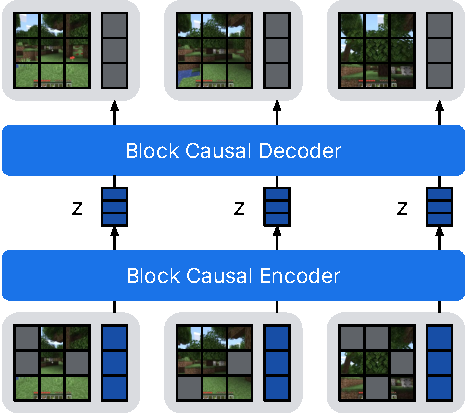
\includegraphics[height=2.4in]{figures/method/tok}
\caption{Causal Tokenizer}
\end{subfigure}%
\hfill%
\begin{subfigure}[t]{0.45\textwidth}
\centering
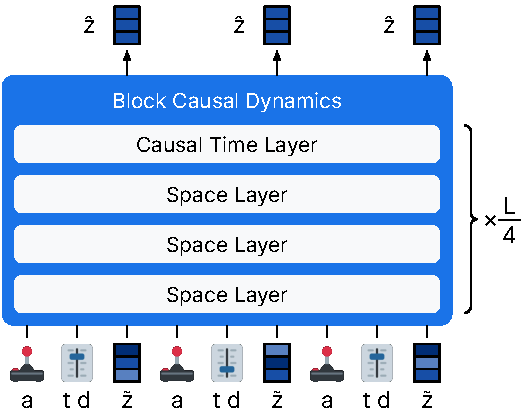
\includegraphics[height=2.5in]{figures/method/dyn}
\caption{Interactive Dynamics}
\end{subfigure}
\caption{World model design.
\method consists of a causal tokenizer and an interactive dynamics model, which both use the same block-causal transformer architecture.
The tokenizer encodes partially masked image patches and latent tokens, squeezes the latents through a low-dimensional projection with tanh activation, and decodes the patches.
It uses causal attention to achieve temporal compression while allowing frames to be decoded one by one.
The dynamics model operates on the interleaved sequence of actions, shortcut noise levels and step sizes, and tokenizer representations.
It denoises representations via a shortcut forcing objective.
After pretraining, the world model is finetuned into an agent by inserting task tokens into the dynamics transformer and predicting actions, rewards, and values from them.
}
\label{fig:model}
\end{figure}

\section{Previous Dreamer Generations}
\vspace*{-1ex}
Dreamer~3\citep{dreamerv3} learned to obtain diamonds in Minecraft from scratch by online interaction.
Its inputs are low-resolution images and inventory states and the outputs are mouse, keyboard, and abstract crafting actions.
Dreamer~3 uses a recurrent state-space model (RSSM) \citep{hafner2018planet} as its world model, which is based on a recurrent neural network and a variational objective.
This approach results in a lightweight world model with highly efficient inference but is difficult to scale to diverse data distributions.
In contrast, \method learns to obtain diamonds in Minecraft purely from offline data.
Its inputs are only high-resolution images and the outputs are low-level mouse and keyboard actions.
\method uses a scalable world model based on an efficient transformer architecture and a shortcut forcing objective, allowing it to scale to diverse data distributions with many details.
While Dreamer~3 uses return normalization and an entropy regularizer, \method uses PMPO with a KL to the behavioral cloning prior for imagination training, where no normalization is needed.
\vspace*{1ex}
\begin{figure}[t!]
\vspace*{-2\baselineskip}
\centering
\begin{subfigure}[t]{0.45\textwidth}
\centering
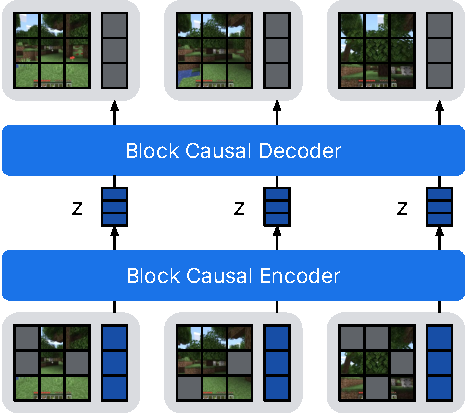
\includegraphics[height=2.4in]{figures/method/tok}
\caption{Causal Tokenizer}
\end{subfigure}%
\hfill%
\begin{subfigure}[t]{0.45\textwidth}
\centering
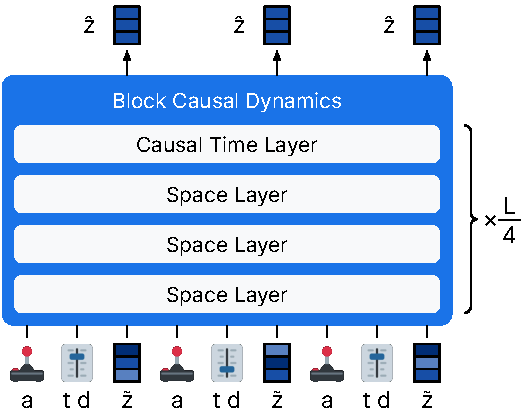
\includegraphics[height=2.5in]{figures/method/dyn}
\caption{Interactive Dynamics}
\end{subfigure}
\caption{World model design.
\method consists of a causal tokenizer and an interactive dynamics model, which both use the same block-causal transformer architecture.
The tokenizer encodes partially masked image patches and latent tokens, squeezes the latents through a low-dimensional projection with tanh activation, and decodes the patches.
It uses causal attention to achieve temporal compression while allowing frames to be decoded one by one.
The dynamics model operates on the interleaved sequence of actions, shortcut noise levels and step sizes, and tokenizer representations.
It denoises representations via a shortcut forcing objective.
After pretraining, the world model is finetuned into an agent by inserting task tokens into the dynamics transformer and predicting actions, rewards, and values from them.
}
\label{fig:model}
\end{figure}
\clearpage

\enlargethispage{\baselineskip}
\vspace*{-10ex}
\section{Human Interaction: Lucid-v1}
\vspace*{-2ex}
\begin{figure}[h!]
% \centering
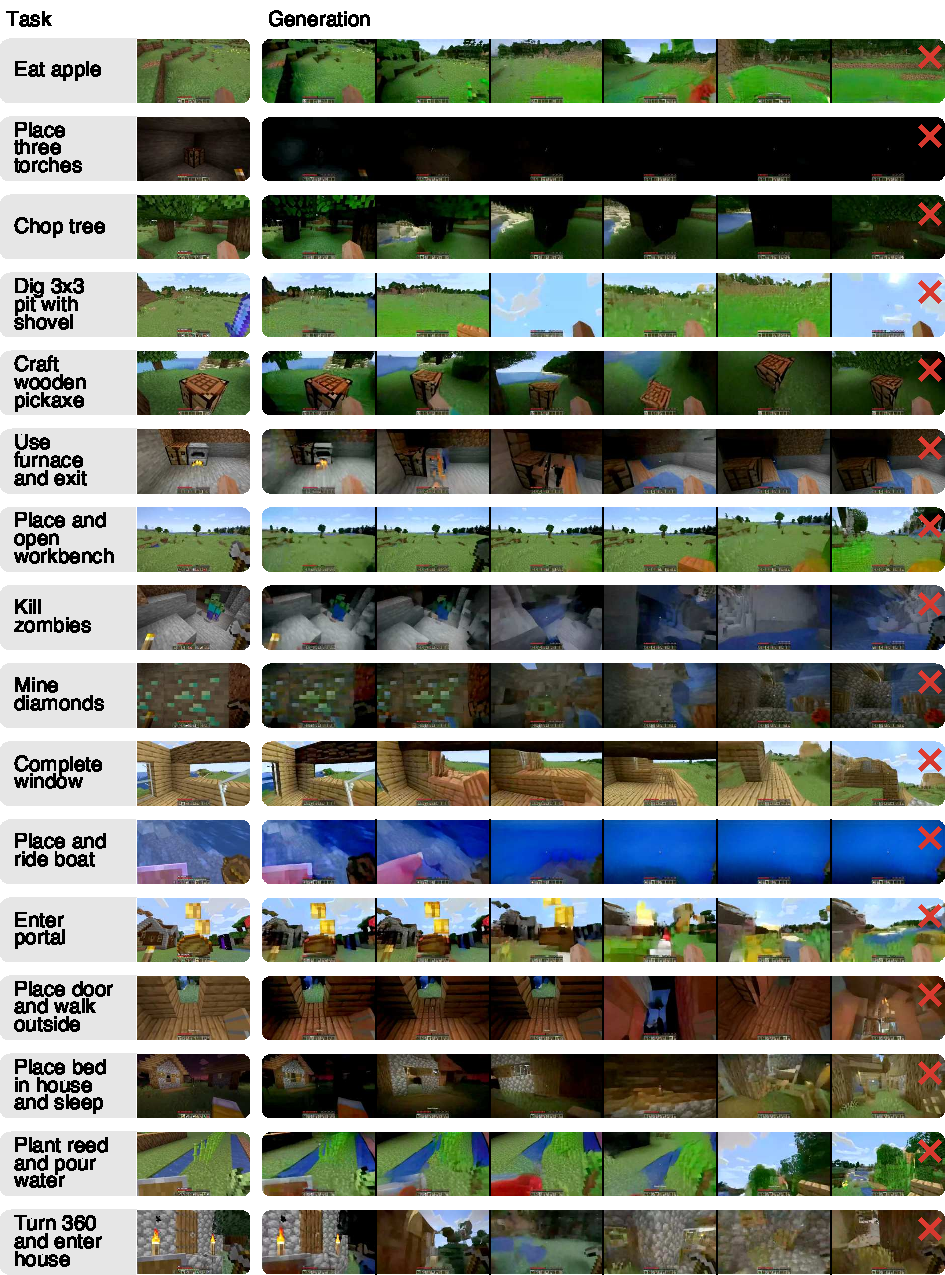
\includegraphics[width=0.97\linewidth]{figures/wmtasks/lucid}
\caption{Lucid-v1}
\label{fig:wmtasks_lucid}
\end{figure}
\vspace*{-2ex}
\clearpage

\enlargethispage{\baselineskip}
\vspace*{-10ex}
\section{Human Interaction: OASIS (large)}
\vspace*{-2ex}
\begin{figure}[h!]
% \centering
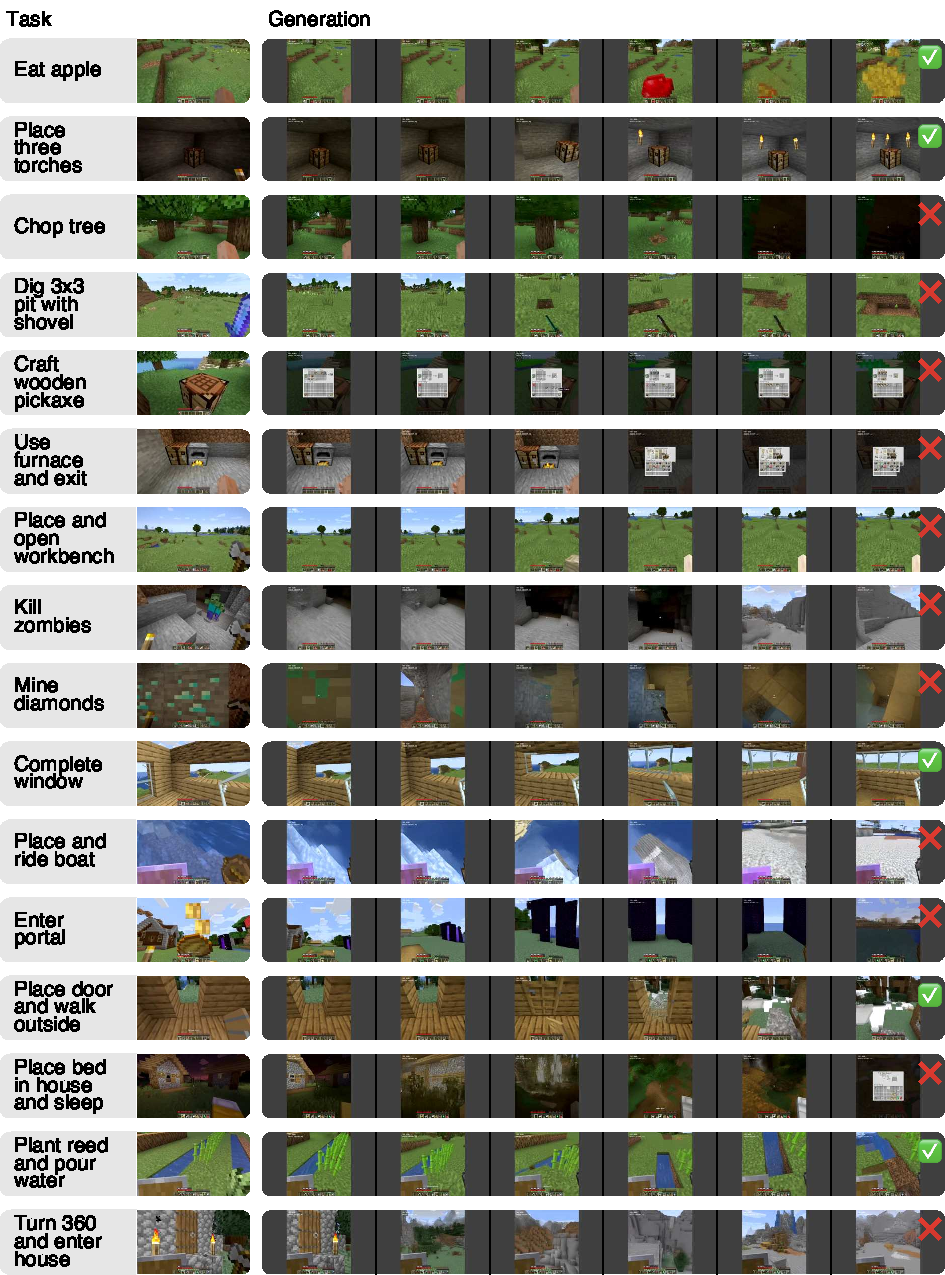
\includegraphics[width=0.97\linewidth]{figures/wmtasks/oasis}
\caption{Oasis (large)}
\label{fig:wmtasks_oasis}
\end{figure}
\vspace*{-2ex}
\clearpage

\enlargethispage{\baselineskip}
\vspace*{-10ex}
\section{Human Interaction: \method}
\vspace*{-2ex}
\begin{figure}[h!]
%\centering
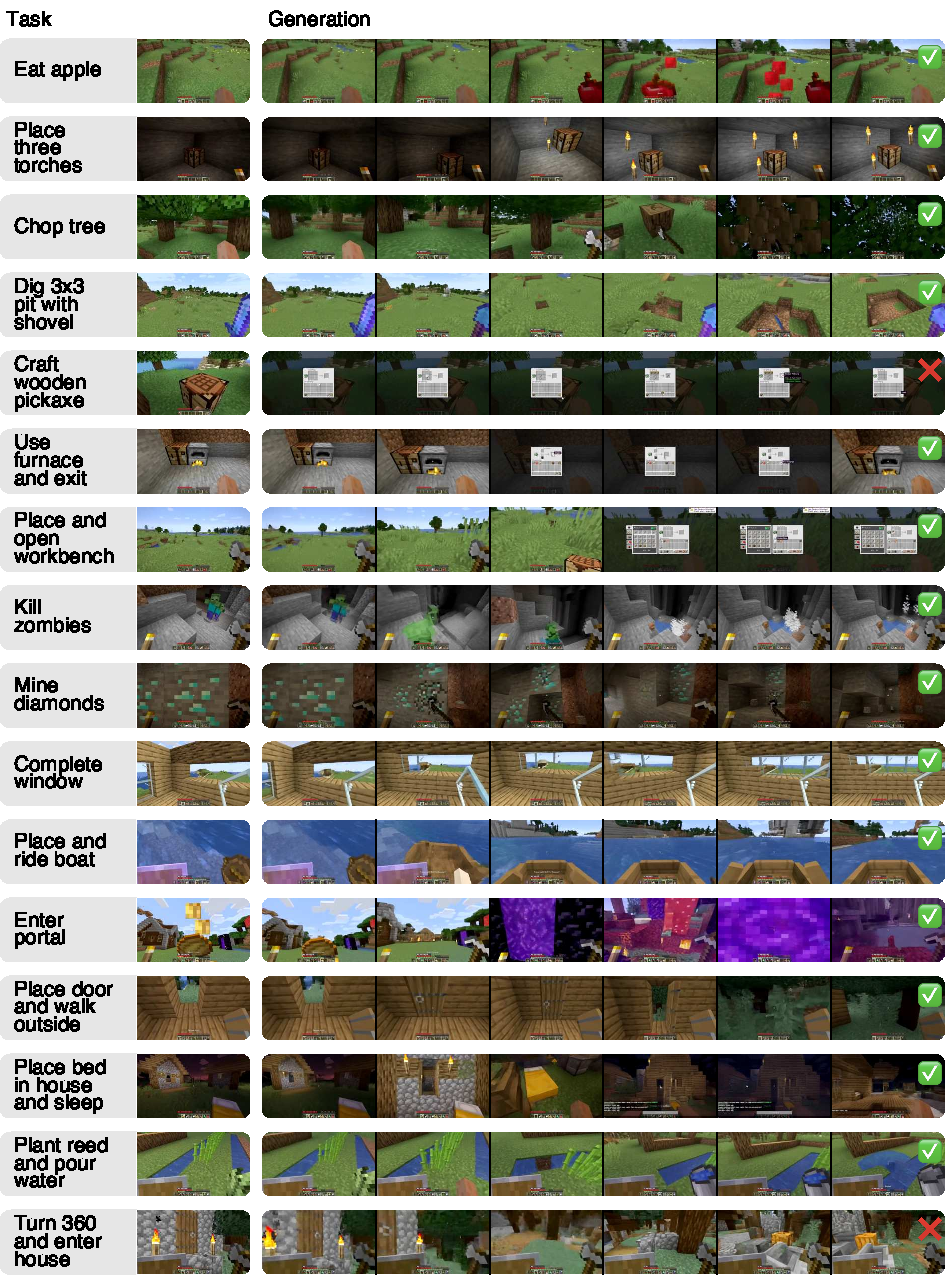
\includegraphics[width=0.97\linewidth]{figures/wmtasks/dreamer}
\caption{\method}
\label{fig:wmtasks_ours}
\end{figure}
\clearpage
